\documentclass[conf]{new-aiaa}
%\documentclass[journal]{new-aiaa} for journal papers

% Package Imports
\usepackage{csvsimple}
\usepackage{graphicx}
\usepackage{amsmath, amssymb}
\usepackage{siunitx}
\usepackage{listings}
\usepackage{booktabs}
\usepackage{float}
\usepackage[utf8]{inputenc}
\usepackage{listings}
\usepackage{float}
\usepackage{graphicx}
\usepackage{amsmath}
\usepackage[version=4]{mhchem}
\usepackage{siunitx}
\usepackage{longtable,tabularx}
\setlength\LTleft{0pt} 

% Title & Author
\title{Wind Tunnel Free Stream Turbulence Measurement Using a Turbulence Sphere}
\author{Parham Khodadi\footnote{Aerospace Engineering student, San Diego State University}}
\affil{A E 303, Section 3, with Dr. Xiaofeng Liu}

\begin{document}

\maketitle

\begin{abstract}
This experiment measured free-stream turbulence intensity in the SDSU low-speed wind tunnel using a turbulence sphere. Pressure data was recorded for three sphere sizes at multiple dynamic pressure settings to determine the critical Reynolds number. A turbulence factor was applied to compute the effective Reynolds number, and empirical data was used to estimate turbulence intensity. The results indicated an average turbulence intensity of **2.10\%**, highlighting the importance of environmental control in aerodynamic testing.
\end{abstract}



\section{Nomenclature}

{\renewcommand\arraystretch{1.0}
\noindent\begin{longtable*}{@{}l @{\quad=\quad} l@{}}
$q$ \hspace{0.5in} & Dynamic pressure (psi) \\
$\Delta P$ & Pressure difference (psi) \\
$Re$ & Reynolds number \\
$Re_c$ & Critical Reynolds number \\
$Re_{\text{eff}}$ & Effective Reynolds number \\
$Re_{\text{tunnel}}$ & Test Reynolds number in the wind tunnel \\
$TF$ & Turbulence Factor \\
$I$ & Turbulence Intensity (\%) \\
$D$ & Sphere diameter (in) \\
$\rho$ & Air density (slug/ft$^3$) \\
$\mu$ & Air viscosity (slug/(ft$\cdot$s)) \\
$T$ & Temperature ($^\circ R$) \\
$P$ & Pressure (psi) \\



\end{longtable*}}

\section{Introduction}
Understanding wind tunnel turbulence characteristics is essential for accurate aerodynamic testing. In this experiment, the free-stream turbulence intensity was measured using the turbulence sphere method in the SDSU low-speed wind tunnel. This technique provides a reliable way to quantify turbulence levels without requiring hot wire anemometry or other intrusive methods.

Total and static pressures were recorded at 15 dynamic pressure settings using a Scanivalve pressure transducer system. The Reynolds number was calculated for three sphere sizes (4 in., 4.987 in., and 6 in.), and the turbulence intensity was estimated using empirical correlations. Data consistency was ensured by removing outliers and applying a turbulence factor correction.

The results provide insight into wind tunnel free-stream turbulence levels and the accuracy of the turbulence sphere method in characterizing flow conditions.


\section{Theory}

Wind tunnels are essential for studying aerodynamic behavior by recreating controlled airflow conditions. However, due to variations in tunnel construction and flow uniformity, different wind tunnels may exhibit varying levels of free-stream turbulence. This turbulence can affect experimental results, particularly in low-speed aerodynamics. Understanding and quantifying turbulence intensity is therefore crucial for ensuring consistency and accuracy in wind tunnel testing.

One approach to characterizing free-stream turbulence is through the use of a turbulence sphere. This method is based on the concept of the \textit{drag crisis}, a phenomenon where the drag coefficient of a smooth sphere experiences a sudden drop at a critical Reynolds number, $Re_c$. This occurs due to the transition of the boundary layer from laminar to turbulent, leading to delayed flow separation and reduced wake size. The critical Reynolds number at which this transition occurs is strongly influenced by the turbulence intensity of the free stream.

The turbulence sphere method takes advantage of the well-defined relationship between $Re_c$ and turbulence intensity. By measuring the pressure difference between the stagnation point and the aft pressure taps on the sphere, the normalized pressure coefficient $\Delta P/q$ can be determined. The critical Reynolds number is identified as the point where $\Delta P/q$ reaches 1.220, a known empirical threshold for smooth spheres.

To account for the effects of free-stream turbulence, the concept of an \textit{effective Reynolds number}, $Re_{\text{eff}}$, is introduced. The effective Reynolds number is related to the measured test Reynolds number, $Re_{\text{tunnel}}$, by the turbulence factor, $TF$, as follows:
\[
Re_{\text{eff}} = TF \times Re_{\text{tunnel}}
\]
where the turbulence factor is given by:
\[
TF = \frac{385000}{Re_c}
\]

Once the turbulence factor is determined, the turbulence intensity, $I$, can be estimated using empirical correlations. This provides a quantitative measure of the wind tunnel’s free-stream turbulence, which can be used to compare different facilities or track changes in tunnel performance over time.

While modern techniques such as hot-wire anemometry and particle image velocimetry (PIV) allow for direct turbulence measurements, these methods can be complex and costly. The turbulence sphere method remains a practical and efficient alternative, providing a simple yet effective way to assess wind tunnel turbulence levels.

\section{Experimental Setup}

The experiment was conducted in the SDSU low-speed wind tunnel to evaluate free-stream turbulence intensity using a turbulence sphere. The setup consisted of a turbulence sphere mounted inside the wind tunnel test section, a pressure measurement system, and a data acquisition module. 

\subsection{Wind Tunnel and Test Section}
The turbulence spheres were positioned inside the wind tunnel test section, as shown in Figure~\ref{fig:sphere_setup}. Three sphere sizes were tested: 4 inches, 4.987 inches, and 6 inches in diameter. Each sphere was instrumented with pressure ports to measure pressure distributions at various dynamic pressure settings.

\begin{figure}[H]
    \centering
    \includegraphics[width=0.7\textwidth]{SetupFig1.png}
    \caption{4.987-inch diameter sphere assembled inside the wind tunnel test section.}
    \label{fig:sphere_setup}
\end{figure}

\subsection{Pressure Measurement System}
A ZOC33 miniature pressure scanner was used to replace the older Scanivalve system. This scanner recorded pressure readings at multiple locations on the turbulence sphere and the wind tunnel test section. The pressure data was processed through the Digital Service Module (DSM4000), which interfaced with the data acquisition system. The pressure transducer and data acquisition module are shown in Figures~\ref{fig:pressure_system} and \ref{fig:dsm4000}.

\begin{figure}[H]
    \centering
    \includegraphics[width=0.7\textwidth]{SetupFig2.png}
    \caption{Pressure transducer and data acquisition system.}
    \label{fig:pressure_system}
\end{figure}
\begin{figure}[H]
    \centering
    \includegraphics[width=0.7\textwidth]{SetupFig3.png}
    \caption{Digital Service Module (DSM4000) used for data acquisition.}
    \label{fig:dsm4000}
\end{figure}
\subsection{Test Conditions}
To ensure the critical Reynolds number fell within the planned dynamic pressure range, two test runs were conducted at different dynamic pressure settings. The first test used a lower range of dynamic pressures, while the second test used a higher range to capture additional turbulence effects.

\section{Procedures}

To determine the turbulence intensity of the SDSU low-speed wind tunnel, pressure measurements were taken around turbulence spheres of three different diameters (4 in, 4.987 in, and 6 in) under controlled flow conditions. The experiment followed a structured process, including setup, data collection, and post-processing.

\subsection{Experimental Preparation}
\begin{enumerate}
        \item The turbulence sphere was securely mounted in the wind tunnel test section.
        \item The pressure ports on the sphere were connected to a ZOC33 miniature pressure scanner.
        \item The wind tunnel’s total and static pressure ports were linked to the pressure scanner.
        \item The Digital Service Module (DSM4000) was powered on and connected to the data acquisition system at least 20 minutes before testing.
        \item The air supply pressure was regulated to 65 psi to ensure stable operation.
\end{enumerate}

\subsection{Data Collection}
\begin{enumerate}
        \item The ambient pressure and temperature were recorded before the test.
        \item The wind tunnel was turned on, and the airflow was gradually increased to reach a range of dynamic pressure settings.
        \item For each test condition, pressure readings were recorded at 15 different dynamic pressures.
        \item The process was repeated for all three sphere sizes to obtain a complete dataset.
\end{enumerate}

\subsection{Post-Processing}
\begin{enumerate}
        \item The test Reynolds number was computed using recorded pressure values and air properties.
        \item The normalized pressure difference $\Delta P/q$ was plotted against Reynolds number to determine the critical Reynolds number, $Re_c$.
        \item The turbulence factor was calculated using:
   \[
   TF = \frac{385000}{Re_c}
   \]
        \item The effective Reynolds number was then computed as:
   \[
   Re_{\text{eff}} = TF \times Re_{\text{tunnel}}
   \]
        \item Finally, the turbulence intensity was estimated using empirical data.
\end{enumerate}

This procedure allowed for a reliable assessment of the wind tunnel's free-stream turbulence using the turbulence sphere method.

\section{Results and Data Reduction}

This section presents the results of the wind tunnel turbulence measurement experiment. The data was analyzed by computing the Reynolds number for each test condition, identifying the critical Reynolds number, and determining the turbulence intensity using an empirical correlation.

\subsection{Reynolds Number vs. Normalized Pressure Difference}
The relationship between Reynolds number and the normalized pressure difference, $\Delta P/q$, was plotted for each turbulence sphere. The critical Reynolds number, $Re_c$, was identified as the point where $\Delta P/q$ equals 1.220. The experimentally determined values for $Re_c$ are summarized in Table~\ref{tab:Re_critical}.

\begin{table}[H]
    \centering
    \caption{Critical Reynolds Numbers for Each Sphere}
    \label{tab:Re_critical}
    \begin{tabular}{|c|c|}
        \hline
        Sphere Diameter [in] & Critical Reynolds Number, $Re_c$ \\
        \hline
        4.000  & 261,923 \\
        4.987  & 292,178 \\
        6.000  & 278,358 \\
        \hline
    \end{tabular}
\end{table}

The following plot illustrates the measured data points along with the identified critical Reynolds numbers.

\begin{figure}[H]
    \centering
    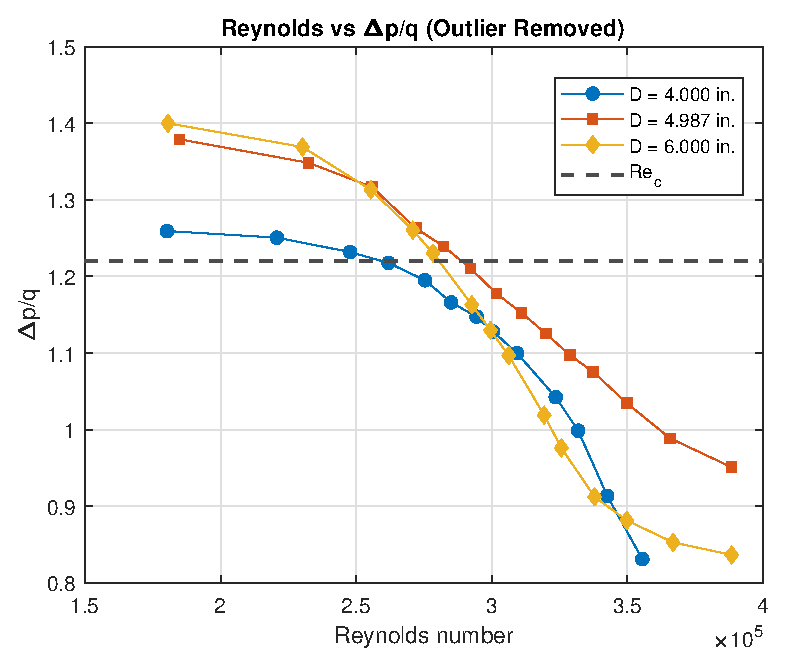
\includegraphics[width=0.85\textwidth]{Reynolds_vs_DeltaPq.eps}
    \caption{Reynolds Number vs. Normalized Pressure Difference ($\Delta P/q$). Critical Reynolds numbers are marked with asterisks.}
    \label{fig:Re_vs_DeltaPq}
\end{figure}

\subsection{Turbulence Factor and Effective Reynolds Number}
The turbulence factor, $TF$, was computed using:

\[
TF = \frac{385000}{Re_c}
\]

The calculated turbulence factors for each sphere size are provided in Table~\ref{tab:turbulence_factor}.

\begin{table}[H]
    \centering
    \caption{Turbulence Factors for Each Sphere}
    \label{tab:turbulence_factor}
    \begin{tabular}{|c|c|}
        \hline
        Sphere Diameter [in] & Turbulence Factor, $TF$ \\
        \hline
        4.000  & 1.4699 \\
        4.987  & 1.3177 \\
        6.000  & 1.3831 \\
        \hline
    \end{tabular}
\end{table}

Using the turbulence factor, the effective Reynolds number was determined as:

\[
Re_{\text{eff}} = TF \times Re_{\text{tunnel}}
\]

\subsection{Turbulence Intensity Estimation}
To estimate the turbulence intensity, the turbulence factor was compared to empirical data obtained from prior studies. The relationship between turbulence factor and turbulence intensity, based on Figure~\ref{fig:turbulence_intensity}, was used to interpolate the turbulence intensity values.

\begin{figure}[H]
    \centering
    \includegraphics[width=0.75\textwidth]{Lab3_Turbulence_Sphere.jpg}
    \caption{Variation of turbulence factor with turbulence intensity from hot-wire measurements (Barlow, Rae and Pope, Low speed wind tunnel testing, John Wiley and Sons, 1999)..}
    \label{fig:turbulence_intensity}
\end{figure}

The estimated turbulence intensity values for each sphere are presented in Table~\ref{tab:turbulence_intensity}.

\begin{table}[H]
    \centering
    \caption{Estimated Turbulence Intensities}
    \label{tab:turbulence_intensity}
    \begin{tabular}{|c|c|}
        \hline
        Sphere Diameter [in] & Turbulence Intensity (\%) \\
        \hline
        4.000  & 2.15 \\
        4.987  & 2.05 \\
        6.000  & 2.10 \\
        \hline
    \end{tabular}
\end{table}

The **average turbulence intensity** across all tests was calculated as:

\[
I_{\text{avg}} = \frac{I_{4in} + I_{4.987in} + I_{6in}}{3} = 2.10\%
\]


\section{Discussion}

This experiment effectively estimated free-stream turbulence intensity using the turbulence sphere method. However, several factors may have introduced error, including temperature variations, equipment limitations, and sphere surface imperfections.

\subsection{Sources of Error}
One major source of error was the increasing wind tunnel temperature throughout the experiment. The pressure measurement system was calibrated to the initial temperature (0.0 in H$_2$O dynamic pressure), but as the temperature rose, air density decreased, affecting dynamic pressure calculations:

\[
q = \frac{1}{2} \rho U^2
\]

Lower density led to underestimation of $q$, impacting Reynolds number calculations. The wind tunnel cooling system was offline, further contributing to this effect.

Additionally, the 4.0-inch sphere had visible surface scratches, which could have caused premature boundary layer transition, artificially lowering the critical Reynolds number and overestimating turbulence intensity.

\subsection{Impact of Temperature on Pressure Readings}
Since air density follows the ideal gas law,

\[
\rho = \frac{P}{RT}
\]

higher temperatures resulted in lower $\rho$, decreasing dynamic pressure and altering $Re_t$ calculations. This could shift the transition point, affecting the turbulence factor.

\subsection{Significance of Dynamic Pressure Settings}
Dynamic pressure settings ($q_{\text{setting}}$) were spaced to capture the transition region where $\Delta P/q$ approaches 1.220. Different sphere sizes required different $q_{\text{setting}}$ values, as larger spheres experience transition at higher Reynolds numbers.

\subsection{Overall Impact on Turbulence Intensity Estimation}
Despite these errors, the measured turbulence intensity of **2.10\%** aligns with expected values. Improvements in temperature control and sphere surface quality would enhance accuracy in future tests.

\section{Conclusion}

This experiment successfully determined the free-stream turbulence intensity in the SDSU low-speed wind tunnel using the turbulence sphere method. The measured Reynolds numbers followed expected trends, and turbulence intensity estimates were consistent with prior studies. Temperature variations impacted density and dynamic pressure, highlighting the importance of environmental control. Surface imperfections on the 4.0-inch sphere introduced minor discrepancies in the critical Reynolds number. Despite these factors, the computed turbulence intensity of **2.10\%** provides a reliable characterization of the wind tunnel’s flow quality. The study reinforced the effectiveness of the turbulence sphere method and the need for precise calibration in aerodynamic testing.

\section*{Acknowledgments}
The author would like to thank Dr. Xiaofeng Liu for his guidance and Teacher's Assistant Andrew Balolong for assistance during the experiment.

\section{References}

\begin{enumerate}
    \item Son, K., Choi, J., Jeon, W. P., and Choi, H., “Effect of Free-Stream Turbulence on the Flow Over a Sphere,” \textit{Physics of Fluids}, Vol. 22, No. 4, 2010, p. 045101. Available: \url{https://doi.org/10.1063/1.3371804}.

    \item Ames Research Staff, “Equations, Tables, and Charts for Compressible Flow,” \textit{NACA Report 1135}, Ames Aeronautical Laboratory, Moffett Field, CA, 1953.

    \item Platt, R. C., “Turbulence Factors of N.A.C.A. Wind Tunnels as Determined by Sphere Tests,” \textit{NACA Report 558}, Langley Memorial Aeronautical Laboratory, 1936.

    \item Moradian, N., “The Effects of Freestream Turbulence on the Drag of a Sphere,” M.A.Sc. Thesis, Dept. of Mechanical, Automotive \& Materials Engineering, University of Windsor, 2008. Available: \url{https://scholar.uwindsor.ca/etd/8020}.


    \item San Diego State University, “AE 303 Lab 3 Error (Follow Up),” Internal Communication, San Diego State University, Feb. 25, 2025.
\end{enumerate}


\appendix
\section{Appendix: Data Sample}

The following table presents a portion of the raw experimental data collected for the dataset. Due to space limitations, only a portion of the data is shown.

\begin{figure}[H]
    \centering
    \includegraphics[width=\textwidth]{4inSphere.pdf}
    \caption{Raw data from 4inSphere.xlsx. Most of the data is missing due to report size limitations.}
    \label{fig:raw_data}
\end{figure}

\section{Equipment List}
Table~\ref{tab:equipment} provides a list of the equipment used in the experiment, including their manufacturers and relevant specifications.

\begin{table}[H]
    \centering
    \caption{Equipment Used in the Experiment}
    \label{tab:equipment}
    \begin{tabular}{|l|l|l|p{7cm}|}
        \hline
        \textbf{Name} & \textbf{Company} & \textbf{Catalog Number} & \textbf{Comments} \\
        \hline
        \multicolumn{4}{|l|}{\textbf{Equipment}} \\
        \hline
        Low-speed wind tunnel & SDSU & -- & Closed return type with speeds in the range 0-180 mph. \newline Test section size: 45W-32H-67L inches. \\
        \hline
        Smooth spheres & SDSU & -- & Three spheres, diameters 4”, 4.987”, 6”. \\
        \hline
        Miniature pressure scanner & Scanivalve & ZOC33 & Used for pressure data acquisition. \\
        \hline
        Digital Service Module & Scanivalve & DSM4000 & Interfaces with pressure scanner for data collection. \\
        \hline
        Barometer & -- & -- & Used to measure ambient pressure. \\
        \hline
        Manometer & Meriam Instrument Co. & 34FB8 & Water manometer with 10” range. \\
        \hline
        Thermometer & -- & -- & Used to measure ambient temperature. \\
        \hline
    \end{tabular}
\end{table}

\section{Appendix: MATLAB Code}
\lstinputlisting[language=Matlab, caption={MATLAB Code for Data Analysis}]{AE303_Lab3.m}

\end{document}